\newpage
\section{Oхорона праці}
Дана дипломна робота передбачає розробку програмного засобу для пошуку у структурах даних гри Го.  Розробка даної програми відбувається в кімнаті офісу на чотирьох осіб, у кожної з яких є робоче місце на один комп’ютер.

Правильно організована робота по забезпеченню безпеки праці підвищує дисциплінованість працівників, поліпшує умови праці, що в свою чергу, призводить до підвищення продуктивності праці, зниження кількості нещасних випадків, запобігання  виходу з ладу обладнання та інших нештатних ситуацій.

Покращення умов праці та її безпека призводить до зменшення виробничого травматизму, професійних хвороб, що зберігає здоров’я працівників та одночасно призводить до зменшення затрат на оплату пільг та компенсацій, на оплату наслідків такої роботи, на лікування, перепідготовку працівників виробництва в зв’язку зі зміною кадрів через причини, що пов’язані з умовами праці.
\subsection{Аналіз робочого місця}
Приміщення, в якому розроблювалася система буде розташоване на другому поверсі п'ятиповерхового будинку та розраховано на чотири робочих місця. Схема приміщення представлена нижче:

\begin{figure}[H]
	\centering
	\caption{Схематичний план приміщення}
	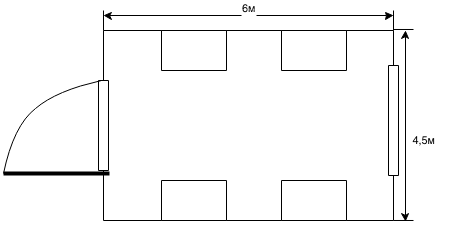
\includegraphics[width=150pt]{safety_room_plan}
	\label{fig:safety_room_plan}
\end{figure}

\begin{tabular}{l}
	Довжина приміщення: 6м;\\
	Ширина приміщення: 4.5м;\\
	Висота приміщення: 3.5м;\\
	Колір підлоги – темний, стін та стелі – світлий.\\
	Коефіцієнти відображення:
\end{tabular}

\begin{equation}
	\rho_\textup{стелі}=70\%,
	\rho_\textup{стін}=50\%,
	\rho_\textup{підлоги}=30\%
\end{equation}

\begin{tabular}{l}
	В приміщенні є одне вікно розмірами: 1.5 м шириною і 2 м висотою.\\
	Площа даного приміщення: $S=6\textup{м}*4.5\textup{м}=27\textup{м}^2$ \\
	Об'єм даного приміщення: $V=S*h=27\textup{м}^2*3.5\textup{м}=94.5\textup{м}^3$\\
	Таким чином, на одне робоче місце надано: $S=6.75\textup{м}^2, V=23.625\textup{м}^3$\\
	Порівняємо розрахункові значення з нормативними у таблиці:
\end{tabular}

\begin{table}[H]
	\centering
	\caption{Розрахункові та нормативні значення площі та об'єму приміщення з розрахунку на одне рабоче місце}
	\begin{tabular}{| l | l | l |}
		\hline
		Параметр приміщення & Нормативний & Розрахунковий\\\hline
		Площа, $\textup{м}^2$ & 6 і більше & 6.75\\\hline
		Об'єм, $\textup{м}^3$ & 20 і більше & 23.625\\\hline
	\end{tabular}
\end{table}

Отже, можна зробити висновок, що площа та об’єм робочого місця відповідає нормам НПАОП 00.0-1.28-10.
\subsection{Аналіз шкідливих і небезпечних факторів}
\subsubsection{Мікроклімат}
Санітарні норми мікроклімату виробничих приміщень в цьому розділі описані згідно ДСН 3.3.6.042-99. Робота, виконувана в даному приміщенні відноситься до категорії робіт – «Легка 1б». У приміщеннях з використанням обчислювальної техніки рекомендується застосування тільки оптимальних значень показників мікроклімату. Нижче приведено видповідні санітарні вимоги до мікроклімату в приміщенні, що повинні дотримуватися.

\begin{table}[H]
	\centering
	\caption{Оптимальні значення параметрів мікроклімату для категорії робіт ``Легка-1б''}
	\begin{tabular}{| l | r | r | r | }
		\hline
		Пора року & Температура, $^oC$ & Вологість, \% & Швидкість повітря, м/с \\\hline
		Тепла & 22-24 & 40-60 & 0,1 \\\hline
		Холодна	& 21-23 & 40-60 & 0,2 \\\hline
	\end{tabular}
	\label{tab:micro-climate}
\end{table}

У приміщенні встановлені батареї центрального водяного опалення, що включається в холодний період року. У теплу пору працює, система кондиціонування, що складається з кондиціонера спліт-системи Кондиціонер DELFA ADW-07C з потужністю 1100 Вт.
\subsubsection{Освітлення}
В приміщеннях для роботи з ЕОМ повинне використовуватися як природне так і штучне освітлення. Природне освітлення забезпечує вікно, загальна площа якого складає $3\textup{м}^2$. Воно являється боковим та одностороннім.

Нормоване значення КПО, яке має забезпечувати природне освітлення розраховується за формулою:

\begin{equation}
	e_\textup{н}=\frac{S_\textup{вік}}{S_n}=\frac{3}{27}=0.11,
\end{equation}

де $e_\textup{н}$ -- значення КПО; $S_\textup{вік}$ -- загальна площа вікна, $\textup{м}^2$; $S_n$ -- площа підлоги, $\textup{м}^2$.

Отримане значення $0.11$ менше ніж встановлено нормами (КПО має бути не меншим за $0.15$), тобто природного освітлення не вистачає для нормальної роботи. Тому потрибно використовувати штучне освітлення.

Штучне освітлення в приміщеннях з робочими місцями, обладнаними ВДТ ЕОМ та ПЕОМ, має здійснюватися системою загального рівномірного освітлення. У якості джерел світла для штучного освітлення мають застосовуватись переважно люмінесцентні лампи типу ЛБ, потужністю 20Вт. Для загального освітлення слід застосовувати 2 світильники серії ЛПО, розташовані у 2 ряди. Один світильник містить 2 лампи, кожна з яких має світловий потік 1060 лм. Нормативна освітленість 300-400 лк., згідно ДБН В.2.6-31. Штучне освітлення кімнати створює освітленість 340 лк, що задовольняє стандарту.
\subsubsection{Шум}
Основним джерелом шуму є системний блок комп’ютера, який містить такі компоненти як: жорсткий диск та кулер.

Таким чином у приміщенні мають місце шуми механічного і аеродинамічного походження. Шум, що створюється, умовно можна віднести до постійного.

Згідно з ДСН 3.3.6.037-99 допустимий шум на постійних робочих місцях користувача складає до 50 дБА. Орієнтовні еквівалентні рівні звукового тиску джерел шуму, що діють на користувача на його робочому місці, представлені в табл. \ref{tab:sound_levels}.

\begin{table}[H]
	\centering
	\caption{Рівні звукового тиску від різних джерел}
	\begin{tabular}{| l | r | }
		\hline
		Джерело шуму & Рівень шуму, дБА \\\hline
		Жорсткий диск & 26 \\\hline
		Кулер & 28 \\\hline
	\end{tabular}
	\label{tab:sound_levels}
\end{table}

Розрахуємо середній рівень шуму на робочому місці користувача при роботі всієї вказаної техніки.

Рівень шуму, що виникає від декількох некогерентних джерел, що працюють одночасно, підраховується на підставі принципу енергетичного підсумовування рівня інтенсивності окремих джерел:

\begin{equation}
	L = 10\lg\sum^n_{i=0}{10^{0.1L_i}},
\end{equation}
де $L_i$ -- рівень звукового тиску і-того джерела.

Підставивши значення рівня звукового тиску для кожного виду устаткування у формулу, отримаємо:

\begin{equation}
	L = 10\lg(4*10^{0.1*26}+4*10^{0.1*28})=36\textup{дБА}.
\end{equation}

Розраховане значення рівня шуму не перевищує гранично допустимого рівня шуму для робочого місця користувача (50 дБА), тобто спеціальні заходи по зниженню рівня шуму не потрібні.

Таким чином, робота з системою, розробленою в дипломній роботі, являється безпечною і не потребує додаткових улаштувань для зниження шуму, окрім загальних методів ізоляції від зовнішнього шуму. Для цього застосовуються  спеціальні віконні профілі та звукоізоляція зовнішніх стін плитами зі звукоізоляційними наповнювачами.
\subsection{Електромагнітні випромінювання}
Більшість учених вважає, що як короткочасна, так і тривала дія всіх видів випромінювання від екрану монітора не небезпечна для здоров'я людини. Проте вичерпних даних щодо небезпеки дії випромінювання від моніторів на людей, що працюють з комп'ютерами не існує і дослідження в цьому напрямі продовжуються.

Допустимі значення параметрів не іонізуючих електромагнітних випромінювань від монітора комп'ютера представлені в табл. \ref{tab:x-ray}.

Максимальний рівень рентгенівського випромінювання на робочому місці оператора комп'ютера звичайно не перевищує 10мкбэр/ч, а інтенсивність ультрафіолетового і інфрачервоного випромінювань від екрану монітора лежить в межах 10-100мВт/м$^2$.

\begin{table}[H]
	\centering
	\caption{Допустимі значення параметрів не іонізуючих електромагнітних випромінювань}
	\begin{tabular}{| l | r | }
		\hline
		Найменування параметра & Допустимі \\\hline
	    Напруженість електричної складової електромагнітного & \\
		поля на відстані 50см від поверхні відеомонітора & 10В/м \\\hline
	    Напруженість магнітної складової електромагнітного & \\
		поля на відстані 50см від поверхні відеомонітора & 0.3А/м \\\hline
		Напруженість поля не повинна перевищувати:  & \\
		для дорослих користувачів & 20кВ/м \\
		для дітей дошкільних установ і що вчаться в & 15кВ/м \\
		середніх спеціальних і вищих учбових закладів & \\\hline
	\end{tabular}
	\label{tab:x-ray}
\end{table}

Для зниження дії цих видів випромінювання рекомендується застосовувати монітори із зниженим рівнем випромінювання (MPR-II, TCO-92, TCO-99, TCO-03), а також дотримувати регламентовані режими праці і відпочинку.
\subsection{Електробезпека}
Робоче місце підпадає під категорію без підвищеної небезпеки тому, що температура у кімнаті не перевищує $30^oC$, вологість не перевищує 60\%, кожен день робиться вологе прибирання.

Електроустаткування належить до приладів до 1000 В. Устаткування, що використовується, відповідно до ПУЄ належить до устаткування класів 0, 0І, і І за електрозахистом.

Оцінка небезпеки дотику до струмових частин відноситься до визначення сили струму, що протікає через тіло людини, і порівняння його із допустимим значенням відповідно до ГОСТ 12.1.038-88.

Лінія електромережі для живлення персональних комп'ютерів, їх периферійних пристроїв (принтер) виконується як окрема групова три-провідна мережа, шляхом прокладання фазового, нульового робочого та нульового захисного провідників. Нульовий захисний провідник використовується для заземлення електроприладів. Провід мідний, ізоляція має бути закритою, марки ПУНП, перерізом не менше 2,5х2мм на жилу. Частота струму не має перевищувати значення 50 Гц.

При виконанні розрахунків для дипломного проекту використовувався персональний комп'ютер - І і II клас захисту, що живиться напругою 220 В. Для правильного визначення необхідних засобів та заходів захисту від ураження електричним струмом необхідно знати допустимі значення напруг доторкання та струмів, що проходять через тіло людини.

Гранично допустимі значення напруги доторкання та сили струму для нормального (безаварійного) та аварійного режимів електроустановок при проходженні струму через тіло людини по шляху ``рука – рука'' чи ``рука – ноги'' регламентуються ГОСТ 12.1.038-88 (табл. \ref{tab:current}).

\begin{table}[H]
	\centering
	\caption{Граничнодопустимі значення напруги доторкання та сили струму, що проходить через тіло людини при нормальному режимі електроустановки}
	\begin{tabular}{| l | r | r |}
		\hline
		Вид струму & В (не більше) & мА (не більше) \\\hline
		Змінний, 50Гц & 2 & 0.3 \\\hline
		Змінний, 400Гц & 3 & 0.4 \\\hline
		Постійний & 8 & 1.0 \\\hline
	\end{tabular}
	\label{tab:current}
\end{table}
\subsection{Пожежна безпека}
Згідно з НАПБ Б.03.002-2007 таке приміщення відноситься до категорії    В–пожежонебезпечна. При нормальному режимі роботи можливість виникнення пожежі мінімальна. Можливість виникнення вибухів повністю відсутня. Можливими причинами загоряння можуть бути пошкодження та замикання в електромережі та електрообладнанні, а також порушення правил безпеки при роботі з обладнанням.

На робочому місці наявні наступні пожежонебезпеці матеріали: папір, пластик, віконні рами, дерев’яні шафи, корпуси техніки, меблі. Робоче приміщення повинно бути обладнане двома вуглекислотними вогнегасниками ВВК-5 з розрахунку два вогнегасника на приміщення  до   25 кв.м  включно, що задовольняє НАПБ Б.03.002-2007. Для захисту від блискавки будівля обладнана блискавковідводом стрижневого типу.

В приміщенні посередині стелі має бути встановлений один димовий пожежний сповіщувач СПД-3 відповідно до ДБН В.1.1.-7-2002 – з розрахунку один на висоту до 3,5 м та загальною площею не більше ніж 86 м$^2$.

Технічні заходи щодо зниження пожежної небезпеки на підприємстві:
\begin{itemize}
	\item застосування засобів пожежогасіння;
	\item використання засобів пожежної сигналізації;
	\item проведення пожежотехнічних обстежень;
	\item використання знаків.
\end{itemize}
